\subsection{Actualización del diseño del código de protocolo}

Primero definimos la estructura de bloques de Nebulas, y luego discutimos cómo actualizar el código de protocolo basándonos en él.

\subsubsection{Estructura de bloques}

La estructura de bloques de datos de Nebulas contiene, pero no se limita a, lo siguiente:\footnote{N. del T.: se preservan los nombres en inglés para la mejor comprensión de los documentos técnicos.}

\begin{itemize}
	\item Header: encabezado de bloque
		\begin{itemize}
		\item Height: altura del bloque
		\item ParentHash: hash del bloque padre
		\item Ts: timestamp
		\item Miner: dirección del minero
		\item Dynasty: \textit{dinastía} del consenso del bloque
		\item Epoch: la \textit{época} del consenso del bloque
		\item StateRoot: hash del estado raíz
		\item TxsRoot: hash de la transacción raíz
		\item ReceiptsRoot: hash del recibo de la transacción
		\item TransNum: número de transacciones
		\end{itemize}
	\item Transactions: datos de la transacción (incluye transacciones múltiples)
		\begin{itemize}
		\item From: dirección del emisor de la transacción
		\item To: dirección del receptor de la transacción, para crear contratos inteligentes se debe usar 0x0
		\item Value: cantidad a transferir
		\item Data: carga útil de la transacción. Si la transacción es para crear un contrato inteligente, contiene su bytecode; si la transacción es una llamada a contrato inteligente, contiene el nombre de la función a llamar.
		\item Signature: firma de la transacción
		\item Gas: límite de gas
		\item GasPrice: precio de la unidad de gas
		\item Nonce: identificador único de la transacción
		\end{itemize}
	\item Votes: preparación y confirmación de votos (incluyendo múltiples), para su uso por el algoritmo de consenso PoD (see \refsec{sec:pod})
		\begin{itemize}
		\item From: votante
		\item VoteHash: hash del bloque votado
		\item Hv: altura del bloque votado
		\item Hvs: altura del bloque padre del votado
		\item VoteType: tipo de voto, Prepare (preparar) o Commit (confirmar)
		\item Signature: firma del voto
		\end{itemize}
	\item Protocol Code: el código del protocolo (dentro de un bloque, tipo binario)
		\begin{itemize}
		\item Hash: hash del código de protocolo
		\item Code: bytecode del código de protocolo
		\item ValidStartBlock: el número del bloque inicial para el cual el protocolo entrará en efecto
		\item Signature: firma (de la comunidad)
		\item Version: número de versión del código del protocolo; cada actualización necesita incrementar este número para prevenir que alguna cuenta maliciosa pueda ejecutar un protocolo obsoleto
		\item Nonce: identificador único del código de protocolo
		\end{itemize}
	\item Nebulas Rank: índice Nebulas (calculado de forma semanal, la mayoría de los bloques no incluyen esta sección)
		\begin{itemize}
		\item RankVersion: versión NR
		\item RankRoot: hash de la valuación NR
		\item RankRecords: registro de la valuación NR
			\begin{itemize}
				\item Address: etiqueta de la dirección de cuenta
				\item Score: valuación NR
			\end{itemize}
		\end{itemize}
\end{itemize}

\begin{figure}[!h]
\centering
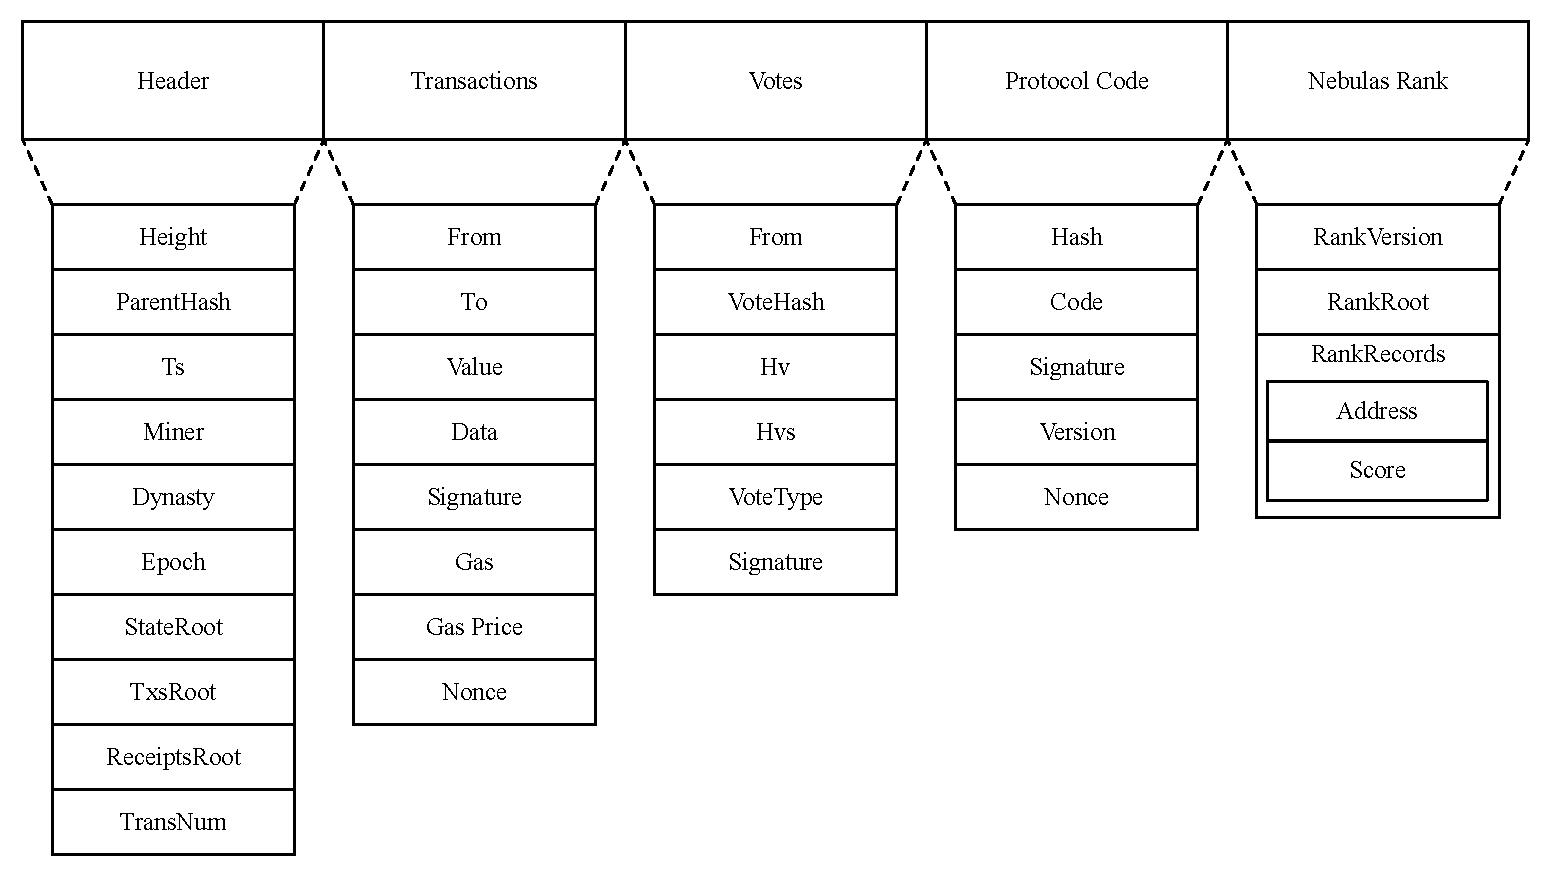
\includegraphics[width=13.8cm]{./figs/block}
\caption{Estructura del bloque}
\label{fig:block}
\end{figure}

De forma similar a otros sistemas de criptodivisa, la interacción entre la cuenta y el blockchain se realiza a través de una transacción en particular. La cuenta crea una transacción, que se firma con una clave privada, la envía a cualquier nodo del blockchain y la transmite al nodo de red completo a través de la red P2P. Durante el intervalo fijo del tiempo de bloque, los nodos especificados por el algoritmo de consenso PoD (ver \refsec{sec:pod}) recogen todas las transacciones en ese lapso, las empaquetan en bloques de formato estándar y las transmiten al resto de la red. Una vez verificado por cada nodo, el nuevo bloque se añade al blockchain local y luego pasa a formar parte del blockchain global.

En Ethereum, las transacciones están divididas en dos tipos: transacciones de cuentas ordinarias y transacciones de contratos inteligentes. En nuestro caso, añadimos dos tipos de transacción nuevos a nuestros bloques: código de protocolo y Nebulas Rank. El código de protocolo, como parte de los datos en el blockchain, se almacenan allí, y la actualización del protocolo básico de Nebulas se lleva a cabo mediante la inserción de datos adicionales en el blockchain. Basado en el algoritmo de valuación NR, el valor NR de cada cuenta se calcula una vez por ciclo y se almacena en el blockchain correspondiente para facilitar la llamada a valores NR en tiempo real, y para realizar consultas históricas.

\subsubsection{Actualización del código del protocolo}

El nodo cliente de Nebulas puede obtener el bytecode compilado de la máquina virtual (NVM bytecode) desde el área de almacenamiento del código de protocolo en el último bloque creado. Si no hay datos del mismo en ese último bloque, significa que el código de protocolo no tiene ninguna actualización, y se debe buscar la versión actual en el bloque más cercano.

Cualquier acción sobre los blockchains será determinada por el código de protocolo, incluyendo el algoritmo de autenticación, las reglas de empaquetado, el algoritmo NR, el mecanismo de incentivos, etc. Casi todas las acciones de los blockchains pueden ser definidas por el código de protocolo.

Si el código del protocolo necesita ser actualizado, el equipo de desarrollo de Nebulas será responsable de su desarrollo y el código será liberado para abrir canales de discusión y votación en las comunidades. La votación se puede llevar a cabo en forma de contrato inteligente o de votación en el foro. Si la mayoría de los miembros de la comunidad están de acuerdo en actualizar el protocolo, el equipo de desarrollo de Nebulas empaquetará el último código en la transacción de código de protocolo, y lo liberará a todos los nodos de la red; una vez que los nodos de contabilidad lo incluyan en bloques, será válido a la altura del bloque especificado. Este tipo de actualización del protocolo en el blockchain es transparente para los clientes sin necesidad de recurrir a \textit{forks}.

Para asegurarse que el código de protocolo se libere después de la autorización, el responsable de su publicación debe utilizar la dirección reservada para el núcleo de Nebulas, que no es modificable en el bloque génesis. Todos los nodos de contabilidad verificarán la firma del código de protocolo. Si la firma no supera la verificación, se considerará que se trata de datos ilegítimos.

La medida de mejora subsiguiente es cambiar la verificación de la firma del código de protocolo por el sistema multifirma M-de-N, que se puede implementar mediante la misma actualización del código de protocolo.